\documentclass[parskip=full]{scrartcl}
\usepackage[utf8]{inputenc} % use utf8 file encoding for TeX sources
\usepackage[T1]{fontenc}    % avoid garbled Unicode text in pdf
\usepackage[german]{babel}  % german hyphenation, quotes, etc
\usepackage{hyperref}       % detailed hyperlink/pdf configuration
\hypersetup{                % ‘texdoc hyperref‘ for options
pdftitle={SWT1: Lastenheftvorlage},%
bookmarks=true,%
}
\usepackage{graphicx}       % provides commands for including figures
\usepackage{csquotes}       % provides \enquote{} macro for "quotes"
\usepackage[nonumberlist]{glossaries}     % provides glossary commands
\usepackage{enumitem}

\makenoidxglossaries
%
% % Glossareinträge
%
\newglossaryentry{Nutzer}
{
	name=Nutzer,
	plural=Nutzer,
	description={(Zahlende) Person welche die Dienste der Applikation nutzt},
}

\newglossaryentry{Abonnament}
{
	name=Abonnament,
	plural=Abonnaments,
	description={Zahlungssystem bei dem der Nutzer monatlich einen festen Betrag zahlt}
}

\newglossaryentry{HDR-Bild}
{
	name=HDR-Bild,
	plural=HDR-Bilder,
	description={(High Dynamic Range Image) Eine Rastergrafik, die große Helligkeitsunterschiede detailreich wiedergibt}
}

\newglossaryentry{Smartphone}
{
	name=Smartphone,
	description={Mobiltelefon mit Touchscreen und zusätzlichen Funktionen wie GPS und der Möglichkeit, Apps darauf zu installieren}
}

\newglossaryentry{Applikation}
{
	name=Applikation,
	description={Als Applikation (kurz App) werden Computerprogramme bezeichnet, die genutzt werden, um eine nützliche oder gewünschte nicht systemtechnische Funktionalität zu bearbeiten oder zu unterstützen}
}

\title{iMage Lastenheft}
\author{Simon Himmel, 2210373}

\begin{document}

\maketitle

%
% % Hinweise - sollen nicht im endgültigen Dokument erscheinen, daher vor der Abgabe löschen!
%


%
% % Hier beginnt die Gliederung des Lastenhefts
%
\section{Zielbestimmung}
Der Benutzer soll durch das Produkt (die \gls{Applikation}) in die Lage versetzt werden, aus seinen eigenen Aufnahmen, gegen bezahlung, HDR-Bilder zu erstellen.

\section{Produkteinsatz}
Das Produkt dient zur erstellung von HDR-Bildern gegen bezahlung. Außerdem sollen diese auch auf sozialen Netzwerken hochgeladen werden können.

Zielgruppe: jeder Nutzer der Applikation.

Plattform: Smartphones mit IOS oder Android Betriebssystem.

\section{Funktionale Anforderungen}
\begin{itemize}[nosep]
\item[FA10] Ersterfassung, Änderung und Löschung von Nutzern (deren Konten).
\item[FA20] Erstellen und Speichern eines HDR-Bildes aus einer Bilderreihe der größe 3.
\item[FA30] Möglichkeit zwischen \gls{Abonnament} und Einzelbild-Preis zu wählen.
\item[FA40] Übersicht über das Nutzerkonto und zuletzt erstellte \glspl{HDR-Bild}.
\item[FA50] Alle Bilder sollen dauerhaft auf dem Zentralserver zur Analyse der Nutzererfahrung gespeichert werden.
\item[FA60] Möglichkeit die \glspl{HDR-Bild} direkt auf sozialen Netzwerken hochzuladen.
\item[FA70] Möglichkeit einer Vorschauansicht der bereits auf dem \gls{Smartphone} gespeicherten Bilder.
\end{itemize}

\section{Produktdaten}
\begin{itemize}[nosep]
\item[PD10] Es sind relevante Daten über die \gls{Nutzer} und deren Konto zu speichern.
\item[PD20] Informationen darüber ob der Nutzer ein Abonnament besitzt.
\item[PD30] Es sind Eingabe- als auch Ausgabebilder dauerhaft auf dem Zentralserver zu speichern.
\end{itemize}

\section{Nichtfunktionale Anforderungen}
\begin{itemize}[nosep]
\item[NF10] Die Funktion /FA20/ darf nicht länger als 7 Sekunden Interaktionszeit benötigen, alle anderen Reaktionszeiten müssen unter 2 Sekunden liegen.
\item[NF20] Es sollen mindestens 1000 Nutzer gleichzeitig mit dem Server kommunizieren können.
\item[NF30] Die Funktion /FA70/ soll in Echtzeit mindestens 100 Bilder auf einem Durchschnittsgerät anzeigen können.
\end{itemize}

\section{Systemmodelle}

\subsection{Szenarien}
Der Nutzer möchte ein HDR-Bild auf seienem Smartphone erstellen. Auf der Startseite der Applikation findes sich bereits erstellte HDR-Bilder und eine Schaltfläche um ein neues HDR-Bild zu erzeugen. Dazu kann er, in einer Vorschau, eine Bilderreihe von seinen eigenen Bildern (bestehend aus 3 Elementen) auswählen. Falls der Nutzer ein Abonamment besitzt kann er direkt das HDR-Bild erstellen, welches dann auf seinem Smartphone gespeichert wird. Ansonsten werden ihm Kaufoptionen angezeigt in denen er dieses Abonnament abschließen kann oder weiterhin einen festen Betrag pro erzeugtem Bild zahlt. Außerdem ist es möglich bereits erstellte HDR-Bilder in einer Vorschau anzeigen zu lassen und diese dann direkt in sozialen Netzwerken zu teilen.
\subsection{Anwendungsfälle}
\begin{itemize}[nosep]
\item Nutzer erstellt HDR-Bild über hochladen seiner 3 Bilder auf Pear-Corp-Zentralserver.
\item Nutzer teilt bereits erzeugte HDR-Bilder in sozialen Netzwerken (z.B Facezine oder Instagrim).
\item Nutzer kann zwischen Abonnament oder Einzelkaufpreis entschgeiden.
\item Speicherung der HDR-Bilder
\end{itemize}
\subsubsection{iMage Model}
\begin{center}
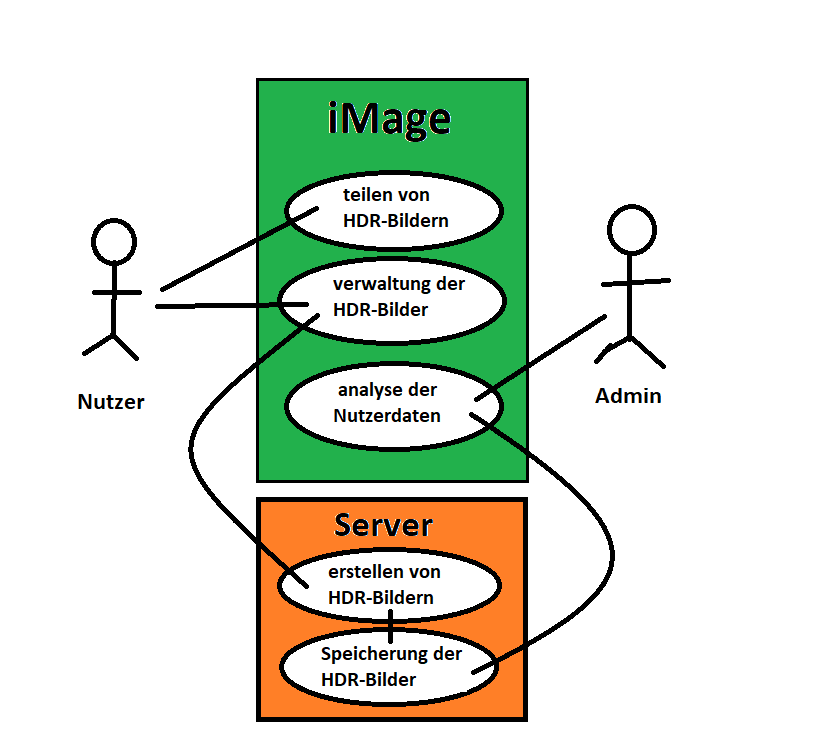
\includegraphics[width=0.8\textwidth]{iMageModel.png}
\end{center}

Akteure: Nutzer, Administrator (Admin).

Anwendungsfälle: HDR-Bild Erzeugung, teilen von HDR-Bilder auf sozialen Netzwerken, Speicherung und Analyse der HDR-Bilder/Daten, 

Textuelle Beschreibung: 

Dem Nutzer ist es möglich über die iMage Applikation seine bereits erstellten HDR-Bilder zu verwalten und mit anderen Leuten im Netz zu teilen. Außerdem kann dieser neue HDR-Bilder erzeugen, welche über den Server erstellt und auch dort gespeichert werden. Dem Administrator ist es nun möglich über iMage auf die Nutzerdaten und über den Server auf alle gespeicherten HDR- und Nicht-HDR-Bilder zuzugreifen und diese zu analysieren.

%
% % Automatisch generiertes Glossar (Latex zwei mal ausführen um Glossar anzuzeigen)
%
%\glsaddall % das sorgt dafür, dass alles Glossareinträge gedruckt werden, nicht nur die verwendeten. Das sollte nicht nötig sein!
\printnoidxglossaries


\end{document}
